% 1983 年全国卷（理科）第 10 题：三棱锥 S-ABC，S 在底面的射影 N 位于底面的高 CD 上，M 是侧棱 SC 上一点，截面 MAB 以浅灰表示（按源卷布局）。
% 源卷图中 S、A、B、C 的连线为实线（可见棱），AC、CD、SN 及截面 MAB 的 MA、MB 两腰为虚线；源卷图无顶点圆点，故不标。
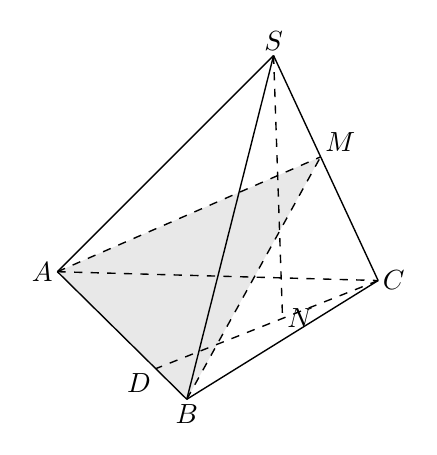
\begin{tikzpicture}[scale=1.0, line width=0.5pt,
  every node/.style={inner sep=1.5pt}]
  \coordinate (S) at (3.245,4.745);
  \coordinate (A) at (0.500,2.000);
  \coordinate (B) at (2.143,0.380);
  \coordinate (C) at (4.573,1.888);
  \coordinate (D) at (1.749,0.769);   % D 在高 CD 的足处，落在 AB 上
  \coordinate (N) at (3.359,1.407);   % N 在 CD 上，且为 S 在底面的射影
  \coordinate (M) at (3.843,3.459);   % M 在侧棱 SC 上
  % 截面 MAB 的浅灰填充
  \fill[gray!18] (A) -- (M) -- (B) -- cycle;
  % 可见棱
  \draw (S) -- (A);
  \draw (S) -- (B);
  \draw (S) -- (C);
  \draw (A) -- (B);
  \draw (B) -- (C);
  % 不可见棱与内部线
  \draw[dashed] (A) -- (C);
  \draw[dashed] (C) -- (D);
  \draw[dashed] (S) -- (N);
  \draw[dashed] (A) -- (M);
  \draw[dashed] (B) -- (M);
  % 顶点与标记点
  \node[above] at (S) {$S$};
  \node[left] at (A) {$A$};
  \node[below] at (B) {$B$};
  \node[right] at (C) {$C$};
  \node[below left] at (D) {$D$};
  \node[right] at (N) {$N$};
  \node[above right] at (M) {$M$};
\end{tikzpicture}
